\documentclass[
	12pt,								% Schriftgröße
	DIV10,
	a4paper,         		% Papierformat
	oneside,						% einseitiges Dokument
%	titlepage,					% es wird eine Titelseite verwendet
	parskip=half,				% Abstand zwischen Absätzen (halbe Zeile)
	headings=normal,			% Größe der Überschriften verkleinern
	listof=totoc,					% Verzeichnisse im Inhaltsverzeichnis aufführen
	bibliography=totoc,						% Literaturverzeichnis im Inhaltsverzeichnis aufführen
	index=totoc,						% Index im Inhaltsverzeichnis aufführen
%	caption=tableheading,	% Beschriftung von Tabellen unterhalb ausgeben
	final								% Status des Dokuments (final/draft)
]{scrartcl}

%--------------------------------------------------------------------------------
% Ab hier werden Packages geladen
\usepackage{lmodern}
\usepackage{caption}
\usepackage[ngerman]{babel}
\usepackage[latin1]{inputenc}
\usepackage[T1]{fontenc}  
\usepackage{amsmath}
\usepackage{blindtext}
\usepackage{ulem} 
\usepackage[latin1]{inputenc}
\usepackage[T1]{fontenc}
\usepackage[ngerman]{babel}
\usepackage{color}
\usepackage{graphicx}
\graphicspath{{./Bilder/}}
\usepackage{subfigure}
\usepackage{cite}
\usepackage{float}
\usepackage{amsmath,amsfonts}
\usepackage{amssymb}
\usepackage{exscale}
\usepackage{subfig} 					
\usepackage{booktabs}
\usepackage{ulem}
\usepackage{setspace}

%für code
\usepackage{listings}
\usepackage{color}
\usepackage{pythonhighlight}

\usepackage[a4paper,lmargin={25mm},rmargin={25mm},tmargin={25mm},bmargin= {25mm}]{geometry}
\addtolength{\footskip}{-0.8cm}		%Fussbereich 0.8cm höher, sodass die Seitennummierung höher ist
\usepackage{tabularx}
\usepackage{tabulary}
\newcolumntype{w}[1]{>{\raggedleft\hspace{0pt}}p{#1}}
\usepackage{eurosym}
\usepackage{siunitx}
\sisetup{exponent-product= \cdot ,output-decimal-marker = {,},detect-family,detect-display-math = true,per-mode = symbol-or-fraction}


\usepackage{lmodern}
\usepackage{fancyhdr} %Paket laden
\usepackage[format=hang]{caption}
\setcapindent{0pt}




\usepackage{listings}
\usepackage{color}
 
\definecolor{codegreen}{rgb}{0,0.6,0}
\definecolor{codegray}{rgb}{0.5,0.5,0.5}
\definecolor{codepurple}{rgb}{0.58,0,0.82}
\definecolor{backcolour}{rgb}{0.95,0.95,0.92}
 
\lstdefinestyle{mystyle}{
    backgroundcolor=\color{backcolour},   
    commentstyle=\color{codegreen},
    keywordstyle=\color{magenta},
    numberstyle=\tiny\color{codegray},
    stringstyle=\color{codepurple},
    stringstyle=\color{codepurple},
    basicstyle=\footnotesize,
    breakatwhitespace=false,         
    breaklines=true,                 
    captionpos=b,                    
    keepspaces=true,                 
    numbers=left,                    
    numbersep=5pt,                  
    showspaces=false,                
    showstringspaces=false,
    showtabs=false,                  
    tabsize=2
}
 

\lstset{numbers=left, numberstyle=\small, numbersep=8pt, frame = single, language=Python, framexleftmargin=1pt, style=mystyle}
%--------------------------------------------------------------------------------
% Hier wird die Titelseite bearbeitet. Im folgenden kommen die zu ändernden Daten
\newcommand{\nameOfTitel}{Projektdokumentation}
\newcommand{\untertitel}{5G \& IIoT Projekt}	% wird nicht verwendet
\newcommand{\art}{Visualisierung der Machine-2-Machine Kommunikation innerhalb einer Webapplikation}
\newcommand{\autor}{Teham Buiyan und Linh Kästner}
\newcommand{\betreuer}{Daniel Nehls}
\newcommand{\datum}{\today}				% hier Abgabedatum einfügen


%-----------------------------------------------------------------------------
\begin{document}

% Ab hier wird die Titelseite zusammengesetzt. Es ist keine Änderung mehr notwendig!
\thispagestyle{plain}
\begin{titlepage}

~\vspace{0.5cm} 
\begin{center}

\includegraphics[width = 0.24\textwidth]{tu-logo_rot}\hspace{2cm} 
  		
\includegraphics[width=0.5\textwidth]{fokus_Logo_930}\hspace{1cm}\\[1cm]
		\Large{TECHNISCHE UNIVERSITÄT BERLIN}\\
			Fakultät IV - Institut für Telekommunikationssysteme\\
			Fachgebiet Architekturen der Vermittlungsknoten
\end{center}

\vspace{1.2cm}
\begin{center}
\LARGE{\textbf{\textsc{\nameOfTitel}}}\\
\LARGE{\textbf{\untertitel}}\\[2ex]
\Large{\textbf{\art}}\\[8ex]

\normalsize
\begin{tabular}{w{5.4cm}p{8cm}}\\
 vorgelegt von:	 & \quad \autor\\[1.2ex]
 Betreuer: & \quad \betreuer\\[1.2ex]
 %Labortermin: & \quad \labortermin\\[1.2ex]
 eingereicht am: &  \quad \datum\\[3ex]
\end{tabular}
\end{center}

\end{titlepage}
\newpage

%-----------------------------------------------------------------------------
\pagenumbering{roman}

%-----------------------------------------------------------------------------
% Eidesstattliche Versicherung der selbstständigen Arbeit
\section*{Eidesstattliche Erklärung}
Wir, \autor, versichern hiermit an Eides statt, dass wir unsere \textsc{\nameOfTitel} - \textit{\untertitel} mit dem Thema
\begin{quote}
\textit{\art}  
\end{quote}
selbständig und eigenhändig angefertigt und keine anderen als die angegebenen Quellen und Hilfsmittel benutzt haben.

\bigskip
\bigskip
\bigskip

Berlin, den \datum


\rule[-0.2cm]{5cm}{0.5pt}

\textsc{\autor} 

\newpage
%-----------------------------------------------------------------------------
\pagestyle{fancy}
\fancyhf{}
\fancyhead[L]{\leftmark}
\fancyhead[R]{Teham Buiyan, Linh Kästner} %Kopfzeile rechts
\fancyfoot[C]{\thepage}
\setlength{\headheight}{8pt}
\renewcommand{\headrulewidth}{0.4pt}
\renewcommand{\footrulewidth}{0.4pt}


\tableofcontents % Inhaltsverzeichnis
\newpage
\pagenumbering{arabic}

%---------------------------------------------------------------------
% Ab hier fängt der eigenständige Teil an!


\section{Einleitung}

Durch den stetigen Fortschritt im Bereich der Informationstechnik, wurden in den vergangenen Jahren innerhalb der Industrie innovative Möglichkeiten in Gang gesetzt. Dabei spielt die Vision von mitdenkenden, sich gegenseitig kontrollierenden Maschinen, eine wichtige Rolle um den Menschen in diversen Aufgaben wie der Wartung oder der Kontrolle von Maschinen zu entlasten und somit den industriellen Gesamtprozess effektiver und sicherer zu gestalten beziehungsweise noch weiter zu automatisieren. Maschinen sollen nicht mehr nur strikten Anweisungen folgen sondern auch mitdenken und selbst agieren können. Dies kann nur auf Grundlage einer sicheren Kommunikation zwischen den Maschinen erfolgen. Diese sogenannte M2M Kommunikation (Maschine zu Maschine) spielt eine essentielle Rolle innerhalb des Industriellen Internets der Dinge und 
als Herausforderung ergeben sich damit diverse Aspekte, welche es zu beachten gilt. 
Zum einen produzieren unterschiedliche Maschinen auch unterschiedliche Datenformate oder arbeiten mit unterschiedlichen Protokollen und Sicherheitstechnologien. Eine Kommunikation kann somit nur mit einer vorherigen Standardisierung geschehen
Die Kommunikation zwischen den Maschinen kann, besonders in einem Anwendungsfall mit mehreren hundert oder sogar tausend Maschinen sehr schnell unübersichtlich werden und die gesamte Netzwerkstruktur verkomplizieren. Ferner sind die Maschinennachrichten so aufzubereiten, dass diese auch für Menschen lesbar ist. Dies ist vor allem für Problembehandlung von enormer Bedeutung.
Es muss sich weiter um die Strukturierung und Aufbereitung der gesammelten Daten gekümmert sowie Plattformen für Anwendungen geschaffen werden, welche es erlauben spezifische Applikationen laufen zu lassen, die jene Maschinendaten verwenden können. Für all diese Probleme wurde die Forschung in den letzten Jahren intensiviert und es ergaben sich diverse Ansätze, welche Grundlage dieses Projektes sind und im weiteren Verlauf näher erläutert werden. 
Ziel des Projektes war es, eine industrienahe Kommunikation zwischen Maschinen zum Zwecke der Übersichtlichkeit und der Effizient bezüglich der Problembehandlung zu visualisieren. Dafür wurde eine Web-basierte Anwendung implementiert, welche es dem Nutzer erlaubt, eine Kommunikation live mitzuverfolgen sowie alle Netzwerkkomponenten zu sehen. Dies stellt einen wichtigen Schritt für die Übersicht und Durchsichtigkeit eines solchen Netzwerkes dar.
\newpage
\section{Theorie}
Bevor das Projekt weiter erläutert wird, sollen auf die wichtigsten Theorieaspekte, welche als Grundlage für das Projekt dienen, eingegangen werden. 
\subsection{Die Verwaltungsschaale}

Die bereits oben genannte Problematik der unterschiedlichen Datenformate und weiteren Aspekten wie der unterschiedlichen Sicherheitsprotokolle und Authentifizierungsstandards wurde durch das relativ aktuelle Konzept der Verwaltungsschale herangegangen. Der Ansatz sieht vor, alle Netzwerkkomponenten mit einer Verwaltungsschale (engl. \textbf{A}dministration \textbf{A}sset \textbf{S}hell (AAS)) auszustatten, welche die unterschiedlichen Datenformate, Funktionen und Protokolle in einem standardisierten Format zur Verfügung stellt und für eine Kommunikation mit anderen Verwaltungsschalen aufbereitet. Somit kann ein Zugriff auf die Daten und Funktionen unterschiedlichster Maschinen erst ermöglicht werden.
Abbildung \ref{func} zeigt exemplarisch Inhalte, welche durch eine Verwaltungsschale bereitgestellt werden können.
\begin{figure}[H]
\centering
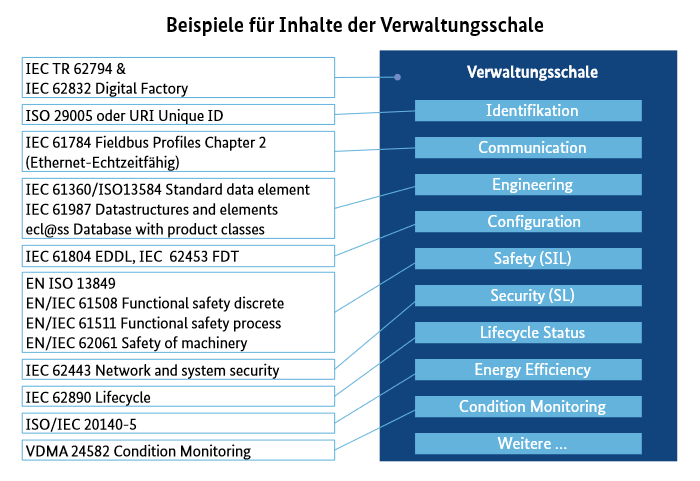
\includegraphics[width=0.8\textwidth]{protos}
\caption{Beispielhafte Inhalte einer Verwaltungsschale (\textbf{Quelle: ZVEI SG Modelle und Standards})}
\label{func}
\end{figure}
Hierin ist zu erkennen, dass die diversen Protokolle für verschiedenste Aspekte wie Sicherheit, Identifikation, Kommunikation oder Energieeffizienz, von der Verwaltungsschale standardisiert bereitgestellt werden muss, um eine konforme Kommunikation mit anderen Verwaltungsschalen zu ermöglichen. 


In Abbildung \ref{struc} ist der detaillierte Aufbau einer Verwaltungsschale zu erkennen.
\begin{figure}[H]
\centering
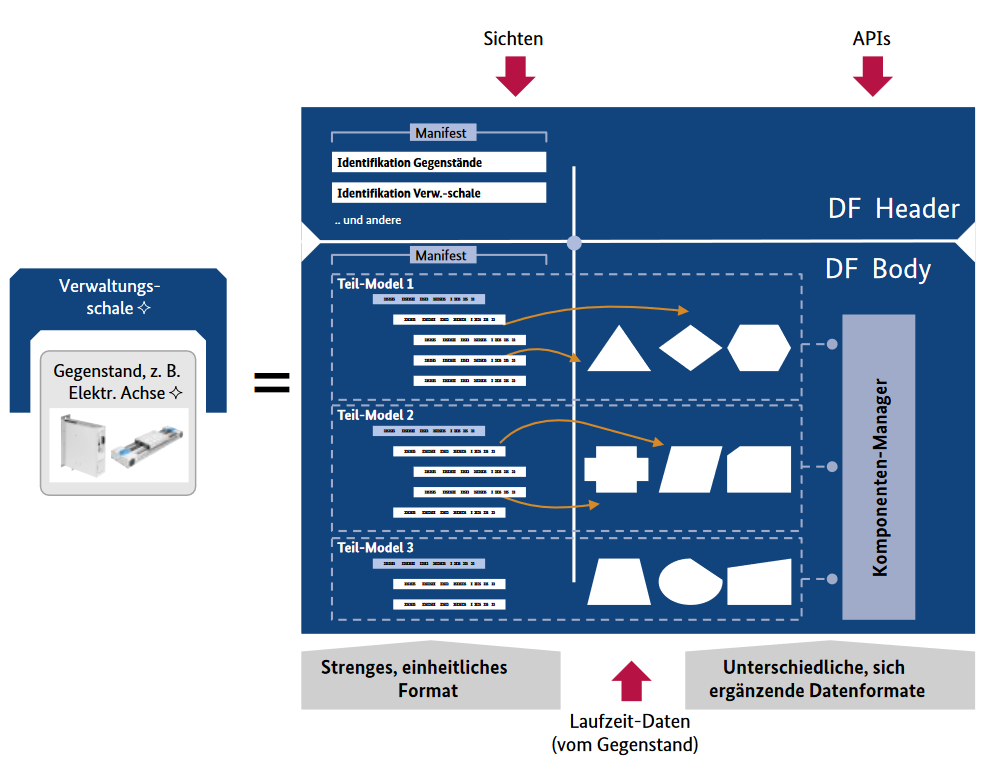
\includegraphics[width=0.8\textwidth]{sturktur}
\caption{Detaillierte Struktur der Verwaltungsschale (\textbf{Quelle: ZVEI SG Modelle und Standards})}
\label{struc}
\end{figure}

Diese besteht aus einem Header und einem Body. Der Header beinhaltet dabei identifizierenden Merkmale der jeweiligen Komponente um damit klar auf Identität und Fähigkeiten der jeweiligen Komponente zu verweisen. 
Der Body enthält dann die spezifischen Teilmodelle zu den verschiedenen Anwendungsfällen/Sichten, welche exemplarisch bereits in Abbildung \ref{func} aufgelistet wurden. Die verschiedenen Datenformate werden im Manifest auf ein strenges, einheitliches Format genormt um einen problemlosen Zugriff durch andere Schalen zu ermöglichen. Die Daten werden dabei mit dem oneM2M Standard genormt, sodass diese für die Nutzung innerhalb einer oneM2M Plattform wie beispielsweise OpenMTC genutzt werden können (Dazu später mehr). Der Komponenten Manager ist für die Verwaltung der verschiedenen Teilmodelle zuständig. Über diesen erfolgt auch der Zugriff auf die spezifischen Daten und Funktionen der Teilmodelle. 


Die wichtigsten Punkte der Verwaltungsschale sind im Folgenden zusammenfassend aufgelistet:
\begin{itemize}
\item Die Verwaltungsschale soll Daten und Funktionen zu verschiedensten Anwendungsszenarien in sogenannten Sichten bereitstellen. Sichten können beispielsweise Angaben zu Bereichen wie Geschäftlich, Leistung, oder Funktionalität sein.
\item Die Verwaltungsschale besteht aus Body und Header.
\item Der Header beinhaltet Identifikationsmerkmale, welche es erlauben auf den Verwendungszweck, mögliche Funktionen  der jeweiligen Komponente zu schließen. 
\item Der Body beinhaltet die detaillierten Untermodelle und den Komponentenmanger, welcher Zugriff auf diese Untermodelle bietet.
\end{itemize}



\subsection{OpenMTC}
Eine auf dem oneM2M Standard basierte Plattform ist OpenMTC, welche am Fraunhofer Fokus entwickelt worden ist. Diese Plattform soll es dem Entwickler erleichtern, anwendungsspezifische Applikationen für die Verwendung innerhalb einer Industrie 4.0 Umgebung zu kreieren. Diese soll Daten von verschiedensten Komponenten über Gateways sammeln und dem OpenMTC Backend zur Verfügung stellen, auf welches wiederum von den Applikationen zugegriffen werden kann. In Abblildung \ref{omtc} ist das Prinzip verbildlicht.

\begin{figure}[H]
\centering
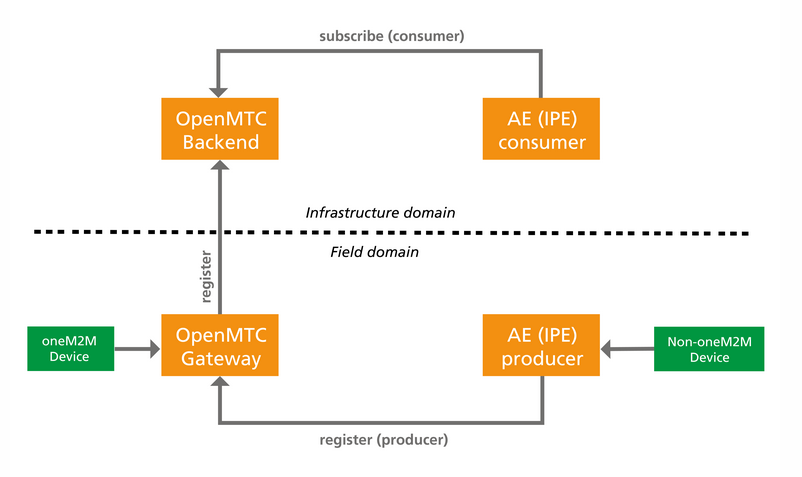
\includegraphics[width=0.8\textwidth]{omtc1}
\caption{OpenMTC Struktur (\textbf{Quelle: openmtc.org)}}
\label{omtc}
\end{figure}

OneM2M-Komponenten werden automatisch erkannt und auf ein Gateway registriert. Durch die im vorigen Kapitel besprochenen Verwaltungsschalen können somit eben solche oneM2M Komponenten erzeugt werden, die automatisch von einem Gateway registriert werden. 

Für die Strukturierung der gesammelten Daten wird das Prinzip der "Containerisation" verwendet, welches es erlaubt, geschachtelte Containerstrukturen zu erstellen, in welchem sich Daten befinden. Diese können nach Belieben mit Labels oder Typen versehen werden, um eine Struktur und Trennung der Daten zu schaffen.
OpenMTC stellt dem Entwickler dafür eine Reihe nützlicher Funktionen zur Verfügung, welche in Tabelle \ref{omtctab} erläutert sind.

\begin{table}[H]
\centering
\label{omtctab}
\begin{tabular}{|l|l|}
\hline
Funktion                                                                                                                     & Beschreibung                                                                                                                                                                                                                                                                                                                                                \\ \hline
\textbf{create\_application}(application, path)                                                                                       & \begin{tabular}[c]{@{}l@{}}Erstellt eine Applikation innerhalb der \\ OpenMTC Umgebung. Unter application \\ muss der Name der App angegeben wer-\\ den. Die Angabe des gewünschten Pfades\\ ist optional.\end{tabular}                                                                                                                                     \\ \hline
\textbf{discover}(path, filter\_criteria)                                                                                             & \begin{tabular}[c]{@{}l@{}}Erkennt zu einem angegeben Elternpfad\\ (path) die zugehörigen Unterpfade und\\ gibt diese innerhalb einer Liste von Adres-\\ sen zurück. Unter filter\_criteria kann zu-\\ dem das Filterkriterium angegeben werden, \\ um spezifische Containeradressen zu \\ erhalten (bspw. alle Container mit \\ Typ 14, etc.)\end{tabular} \\ \hline
\begin{tabular}[c]{@{}l@{}}\textbf{create\_container}(target, container,\\ labels)\end{tabular}                                       & \begin{tabular}[c]{@{}l@{}}Erzeugt einen Container innerhalb der \\ Ressourcen Struktur. Nach Wunsch können\\ diese mit Label versehen werden und ange-\\ geben werden wieviele Container maximal\\ angezeigt werden sollen.\end{tabular}                                                                                                                   \\ \hline
\textbf{push\_content}(container, content)                                                                                            & \begin{tabular}[c]{@{}l@{}}Sendet Daten (content) an einen Container\\ (container). Dabei können als Daten Python \\ Strings, Listen oder Dictionaries gesendet\\ werden.\end{tabular}                                                                                                                                                                      \\ \hline
\textbf{get\_content}(container)                                                                                                      & Ruft Daten aus einem Container ab.                                                                                                                                                                                                                                                                                                                          \\ \hline
\begin{tabular}[c]{@{}l@{}}\textbf{add\_container\_subscription}(container, \\ handler, data\_handler, filter\_criteria)\end{tabular} & \begin{tabular}[c]{@{}l@{}}Subskription auf einen container, um auto-\\ matisch die aktuellsten Daten dieses Con-\\ tainers zu erhalten. Mit filter\_criteria kann \\ auf spezifische Container innerhalb der\\ Containerstruktur subskribiert werden.\end{tabular}                                                                                         \\ \hline
\textbf{emit}(message, event)                                                                                                         & \begin{tabular}[c]{@{}l@{}}Sendet Daten(message) via Websockets an\\ das Frontend. Event ist dabei der "Kanal" \\ auf welchem gesendet wird. Von Frontend \\ Seite kann durch Angabe diesen Kanals, \\ darauf gelauscht werden, um Daten\\ automatisch zu bekommen\end{tabular}                                                                             \\ \hline
\end{tabular}
\caption{wichtige OpenMTC Funktionen}
\end{table} 
Obige Funktionen wurden im Projekt verwendet, um Daten in Container zu lagern 
\begin{itemize}
\item \textbf{push\_data()}
\end{itemize} 
und aus Containern zu erhalten
\begin{itemize}
\item \textbf{get\_content(), add\_container\_subscription()}
\end{itemize} 
Weiterhin sind Funktionen von Relevanz, welche die Adressen spezifischer Container zurückgeben
\begin{itemize}
\item \textbf{discover()}.
\end{itemize} 
\subsection{RDF und JSON-LD}
Das RDF-Modell (englisch für Ressource Description Framework) beschreibt, wie der Name bereits vermuten lässt, ein Konzept zur Formulierung und Beschreibung von Ressourcen innerhalb des Internets. Das Konzept beruht auf Graphen, welche eine Ansammlung von Aussagen über diese Ressourcen sind. Jene Aussagen werden immer als Triple formuliert, welche die Ressource näher beschreiben soll. Dabei ist die Ressource um die es geht das Subjekt, das durch ein Prädikat in Verbindung zum Objekt gebracht wird. 
Um das RDF Konzept zu serialisieren, also in einem speicherfähigem Format einzubetten, wird üblicherweise JSON-LD (JSON-Linked Data) genutzt. JSON-LD gibt als Erweiterung zum JSON-Format, den Informationen einen Kontext und eine Identifizierung, womit Daten von Maschinen leichter in einen gedeutet und verstanden werden können. Außerdem sind Informationen zu einem Subjekt durchweg mit anderen Informationen vernetzt, womit ein Subjekt durch Vernetzungen zu weiteren Informationen näher beschrieben werden kann. Abbildung \ref{rdf} verbildlicht dies an einem Beispiel.

\begin{figure}[H]
\centering
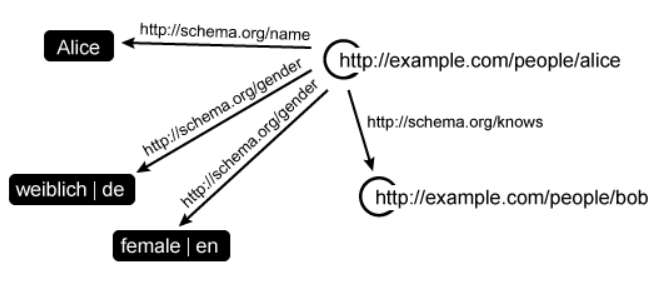
\includegraphics[width=0.8\textwidth]{rdf}
\caption{Beispiel eines Graphen nach dem RDF-Modell (\textbf{Quelle: w3.org/TR/json-ld})}
\label{rdf}
\end{figure}
Subjekt und Prädikat stellen die Knoten im Graphen dar, während die Prädikate die Kanten im Graphen sind. Subjekt und Prädikat sollten dabei eindeutige Adressen (IRIs) beinhalten wobei ein Objekt entweder eine weitere (IRI) beinhalten kann (die dann aufgelöst, weitere Informationen gibt) oder ein Text zur Beschreibung ist.
In obigen Beispiel ist das Subjekt die Person Alice, welche durch die eindeutige Adresse zum Typ 'people' gehört. Dieses Subjekt ist, über die Prädikate 'gender', 'name' und 'knows' mit diversen Objekten vernetzt. In den Adressen der Objekte, befinden sich weitere Informationen, wie eine Spezifizierung, dass 'gender' eines von 2 Geschlechtern bei Menschen ist und dieses in unterschiedlichen Sprachen dargestellt werden kann. Ein Objekt kann dabei auch eine weitere IRI enthalten, wie beispielsweise die Person Bob, welche aufgelöst weitere Informationen enthält.
\newpage
\subsubsection*{Maschinennachrichten}
Auch die im Projekt erzeugten Maschinennachrichten wurden mit dem JSON-LD Format serialisiert. Ebenfalls liegt das Turtle Format vor, welches dieselbe Information in einer leichter verständlichen Syntax darstellt, vor, weswegen im Folgenden auf eine solche Nachricht zur Selektion einer blauen Schokolade an den Roboter, eingegangen wird. 


\begin{lstlisting}
@prefix ns1: <http://www.vendor.com/rdf/> .
@prefix ns2: <http://www.fokus.fraunhofer.de/ontologies/i40/> .

ns1:Message3CTF3N a ns2:Message ;
    ns2:RID "/robot-cse/onem2m" ;
    ns2:SID "/ip-cse-1/onem2m" ;
    ns2:StepNumber "1" ;
    ns2:TID ns2:T20000 ;
    ns2:TRN "http://www.fokus.fraunhofer.de/ontologies/i40/T20000" ;
    ns1:color "blue" .
\end{lstlisting}

Die Prefixe geben analog zum vorherigen Beispiel, den Kontext eines Subjekts oder Objekts an. In diesem Falle ist das Subjekt die Nachricht 'Message3CTF3N', die vom Typ Message ist. Dieser Typ wird weiter in den Code Zeilen 5 bis 10 weiter spezifiziert. Hierin ist zu erkennen, dass der Typ 'Message' über Informationen wie RID, SID, etc. verfügt, auf die bei Bedarf zugegriffen werden kann. Der Graph einer solchen Nachricht kann analog zum Beispiel oben mit Abbildung \ref{rdfm} dargestellt werden.

\begin{figure}[H]
\centering
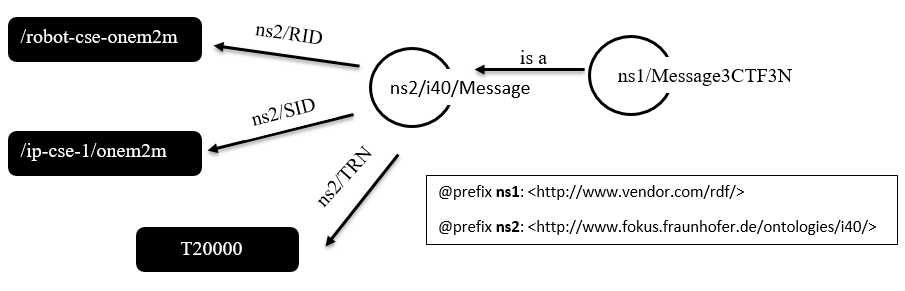
\includegraphics[width=0.95\textwidth]{rdfmessage}
\caption{Graph einer Maschinennachricht}
\label{rdfm}
\end{figure}

Für das Projekt von Relevanz ist, die Informationen aus einem solchen Graphen zu extrahieren. Dazu stellt die 'RDF-Bibliothek' folgende Funktionen zur Verfügung:

\begin{table}[H]
\centering
\label{my-label}
\begin{tabular}{|l|l|}
\hline
Funktion                                                           & Beschreibung                                                                                                                                                              \\ \hline
\textbf{Graph}()                                                            & \begin{tabular}[c]{@{}l@{}}Erstellt eine Graph-Variable, in die ein\\ Graph eingebettet werden kann\end{tabular}                                                          \\ \hline
\textbf{parse}(data, format)                                                & \begin{tabular}[c]{@{}l@{}}Bettet einen Graphen (data) in eine Variable\\ ein. Als zweites Argument wird das Format\\ des Graphen angegeben (z.B.: JSON-LD).\end{tabular} \\ \hline
\begin{tabular}[c]{@{}l@{}}\textbf{value}(predicate,\\ object)\end{tabular} & \begin{tabular}[c]{@{}l@{}}Entnimmt dem Graphen den entsprechenden\\ Wert des angegebenen Objektes.\end{tabular}                                                          \\ \hline
\end{tabular}
\caption{Funktionen der RDF Bibliothek}
\end{table}

 
\subsection{Websockets}
Websockets sind eine effiziente Möglichkeit, Daten bidirektional in Echtzeit zwischen Backend (Webserver)- und Frontend (Webapp) auszutauschen. Dazu wird für eine Verbindung ein sogenanntes Socket (Sockel/ Verbindung) erstellt und es werden Daten auf einen bestimmten Kanal gesendet. Auf diesen Kanal kann von Frontend Seite aus 'gelauscht' werden, was einer Art Subskription gleichkommt. Die Verbindung ist dabei immer aktiv, sodass, im Gegensatz beispielsweise zu einem HTTP - Request, nicht jedes mal eine Anfrage gesendet werden muss. Somit muss kein Polling (kontinuierliches Abfragen) betrieben werden und aktuelle Daten werden in Echtzeit zum Frontend gesendet. Abbildung \ref{setup2} verbildlicht oben genannten Vergleich.

\begin{figure}[H]
\centering
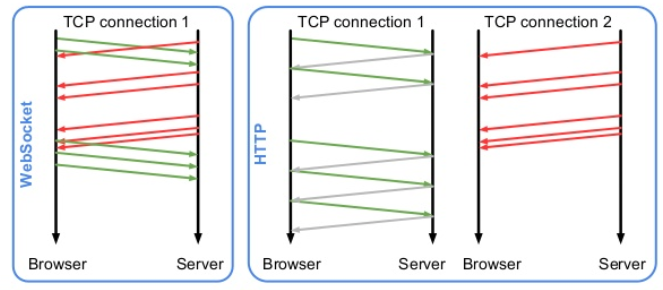
\includegraphics[width=0.8\textwidth]{socket}
\caption{Websockets vs. HTTP-Anfragen (\textbf{Quelle: devcentral.f5.com})}
\label{setup2}
\end{figure}
Während bei Websockets eine Bidirektionale Verbindung vorherrscht, benötigt eine HTTP Anfrage mindestens 2 Verbindungen um Daten austauschen zu können. 
Durch diese Eigenschaft eigenen sich Websockets besonders gut für einen Chat-Raum, welcher auch Ziel des Projektes ist.
Zur Verwendung von Websockets wurde im Projekt dabei die 'socket.io' Bibliothek benutzt. Im Folgenden soll kurz auf die Verwendung eingegangen werden.

\subsubsection*{Verwendung von Websockets mit socket.io}
Mit 
\begin{lstlisting}
socket = io()
\end{lstlisting}
wird ein Socket erstellt. Wurden nun vorher auf Backend Seite mit 
\begin{lstlisting}
emit('message',data)
\end{lstlisting}
Daten auf den Kanal 'message' gesendet, so kann mit 
\begin{lstlisting}
socket.on('message', function(data){...}
\end{lstlisting}
eine Verbindung hergestellt und auf diesen Kanal gelauscht werden. Innerhalb dieser Funktion kann wird dann die Routine gestartet.



\newpage



\section{Setup und Motivation}
\subsubsection*{Setup}
Das Setup besteht aus drei Komponenten, welche jeweils mit einer AAS ausgestattet sind und somit vollständige Komponenten im OpenMTC Netzwerk sind. Diese können miteinander interagieren und kommunizieren um eine gewünschten Prozess automatisch zu bearbeiten. Konkret geht es um die Bestellung von verschiedenfarbiger Schokolade, welche durch eine GUI (ChoclateGUI) getätigt werden kann. Die Box (Intelligent Product) empfängt nach tätigen der Bestellung in der Chocolate-GUI die Informationen von der GUI und gibt diese an das Laufband weiter. Das Laufband erkennt anhand des Headers, die notwendigen Befehle und gibt diese an den Roboter weiter. Dieser beginnt dann mit der Abarbeitung der Bestellung. Ist diese beendet gibt der Roboter eine Notifikation an das Laufband, womit dieses automatisch weiter fährt. Ein Demo Video ist auf Anfrage verfügbar und veranschaulicht den Gesamtprozess. In Abbildung \ref{setup} ist das Setup verbildlicht. 

\begin{figure}[H]
\centering
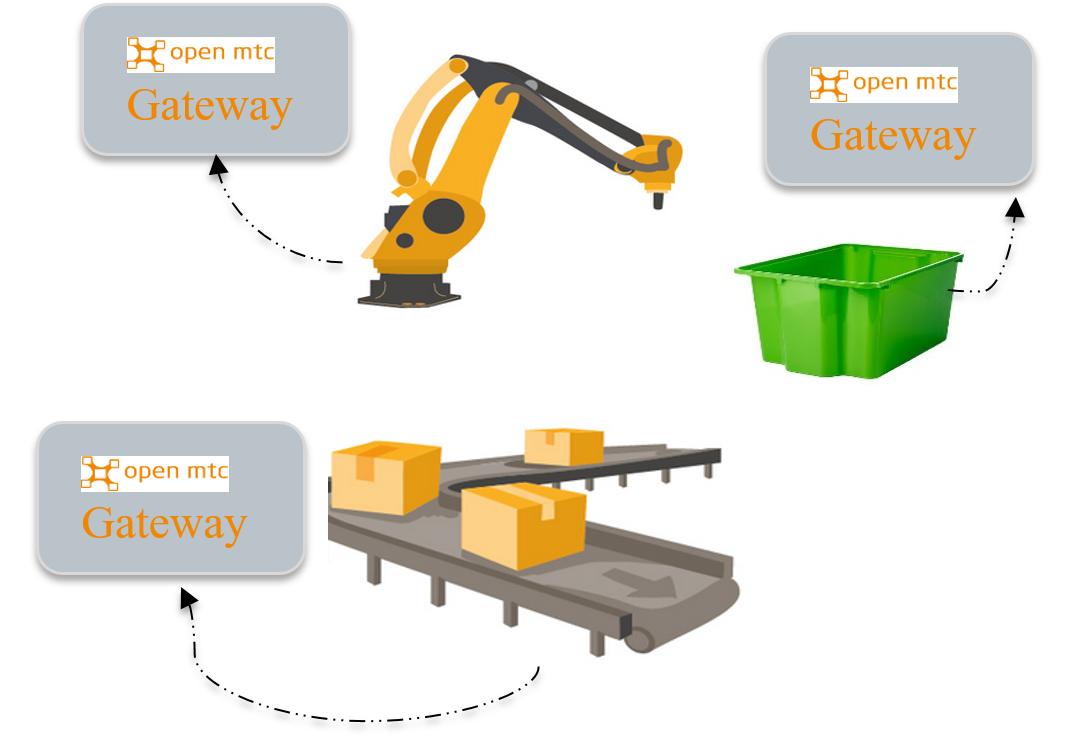
\includegraphics[width=0.8\textwidth]{setup}
\caption{Setup \textbf{(Bildquellen: the-mtc.org, iot.do)}}
\label{setup}
\end{figure}

Dort sind die drei erwähnten Komponenten zu sehen, welche die produzierten Daten/Nachrichten an das jeweilige Gateway (die AAS) senden. Die Daten/Nachrichten werden dabei im JSON-LD Format gesendet. Somit befindet sich, wie bereits schon in der Theorie präsentiert, in einer Maschinennachricht u.a. stets die Information über den Absender, den Empfänger und die Nachricht, auf welche von jedem anderen OpenMTC Gateway zugegriffen werden kann. Dazu werden Funktionen der OpenMTC Plattform benutzt, wobei der detaillierte Ablauf und die Verwendung dieser Funktionen im Kapitel 'Implementierung - Backend' erläutert wird.
Da die produzierten Daten an drei verschiedene Gateways gesendet werden, muss es Filterkriterien geben, welche eine Gruppierung der verschiedenen Gateways erlaubt. Dazu wird eine Containerstruktur angelegt, welche es ermöglicht Daten strukturiert und mit Kriterien wie Label oder Typ zu versehen um dann durch die Vergabe von gleichen Labels oder Typen auf alle relevanten Gateways zuzugreifen.

\subsubsection*{Motivation}
Die Visualisierung der Kommunikation zwischen den einzelnen Komponenten ist aufgrund diverser Aspekte, ein wichtiger Faktor, welcher noch nicht realisiert wurde. Dementsprechend war die Aufgabe eine solche Visualisierung zu implementieren. Dies hat durch folgende Punkte große Relevanz: 
\begin{itemize}
\item Die Sichtbarkeit der Kommunikation fördert die Durchsichtigkeit des Netzwerkes. Somit kann der Betrachter der Kommunikation zwischen den Maschinen folgen und nachvollziehen. Dies ist vor allem für die Problembehandlung von hoher Bedeutung. 
\item Die Aufbereitung der schwer lesbaren Maschinennachrichten, erleichtert die Administration und trägt zu einer deutlich erhöhten Verständlichkeit des Prozesses, auch für Außenstehende, bei. Außerdem wird dadurch die Administration effektiver.
\item Die Sichtbarkeit der Komponenten innerhalb des Netzwerkes fördert ebenfalls die Übersichtlichkeit des Netzwerkes. Dies geschieht vor allem im Hinblick auf ein deutlich komplexeres Netzwerk mit mehreren hundert Komponenten. Somit hat der Betrachter eine Übersicht über die im Netz befindlichen Geräte, was weiterhin ebenfalls in einer höheren Effektivität bei der Administration solcher Netzwerke resultiert. 
\end{itemize}

\section{Zielstellung}
Die angestrebten Ziele können nach obiger Motivation wie folgt definiert werden:
\begin{itemize}
\item Erstellung einer Webbasierten Applikation zur Visualisierung der Maschinenkommunikation .
\item Aufbereitung der Maschinennachricht zu einer übersichtlichen, auch für Außenstehende, verständlichen Form.
\item Anzeige der Komponenten, welche sich innerhalb des Netzwerkes befinden.
\item Erstellung eines ansprechenden Designs mit Personalisierungsmöglichkeiten
\item Möglichkeit weitere Funktionen in die Web Applikation zu integrieren
\end{itemize}

\newpage




\section{Konzeption}
\subsubsection*{Backend}
Wie bereits oben erwähnt, werden die Daten der drei Komponenten an ihre jeweiligen Gateways gesendet. Durch gleiche Labels können diese drei Gateways bildlich als ein Gateway dargestellt werden, wie dies in Abbildung \ref{concept} geschehen ist. Für das Empfangen und die Aufbereitung der Daten aus dem Gateway ist ein Backend in Form einer Python App notwendig. Wichtig ist dabei, dass dies mittels des OpenMTC App Frameworks (Funktion create\_application()) erstellt werden muss um eine richtige Ordnerstruktur zu schaffen und somit eine fehlerfreie Funktionalität zu gewährleisten. Die Auslagerung und Aufbereitung der Daten im JSON Format passiert ebenfalls primär mit den besprochenen Funktionen des OpenMTC Frameworks, das anschließende Senden geschieht mittels Websockets, wobei hier auf Frontend Seite die Socket.io Bibliothek benutzt wurde. 


%\begin{figure}[H]
%\centering
%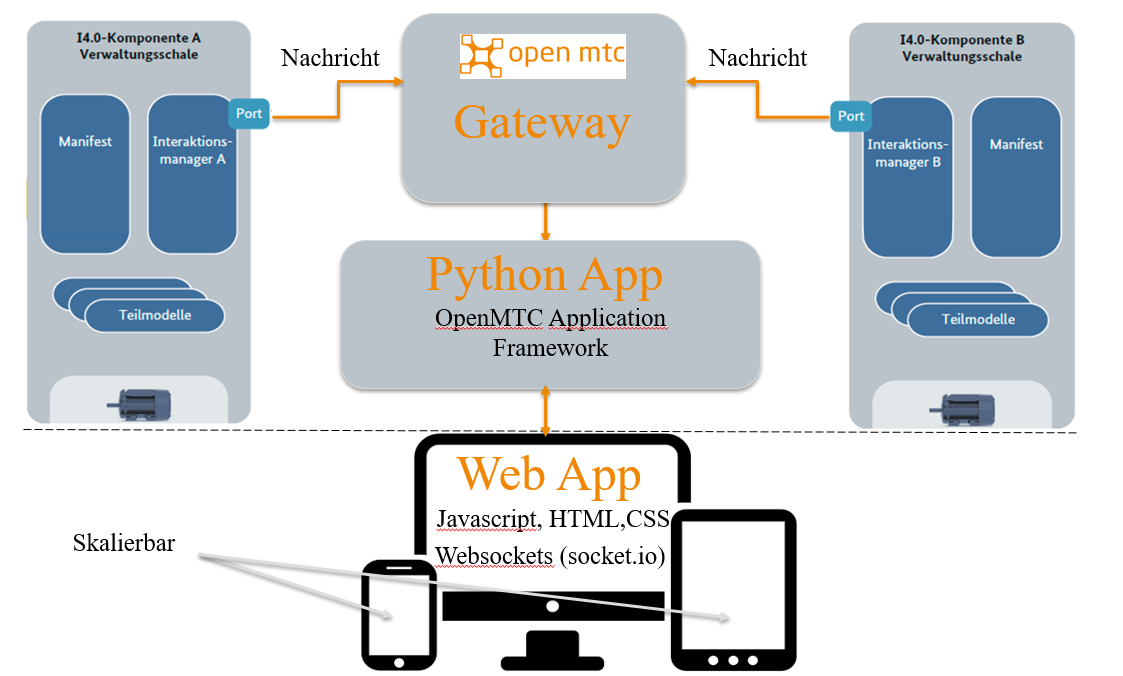
\includegraphics[width=0.9\textwidth]{idee}
%\caption{Konzeption}
%\label{setup}
%\end{figure}

\begin{figure}[H]
\centering
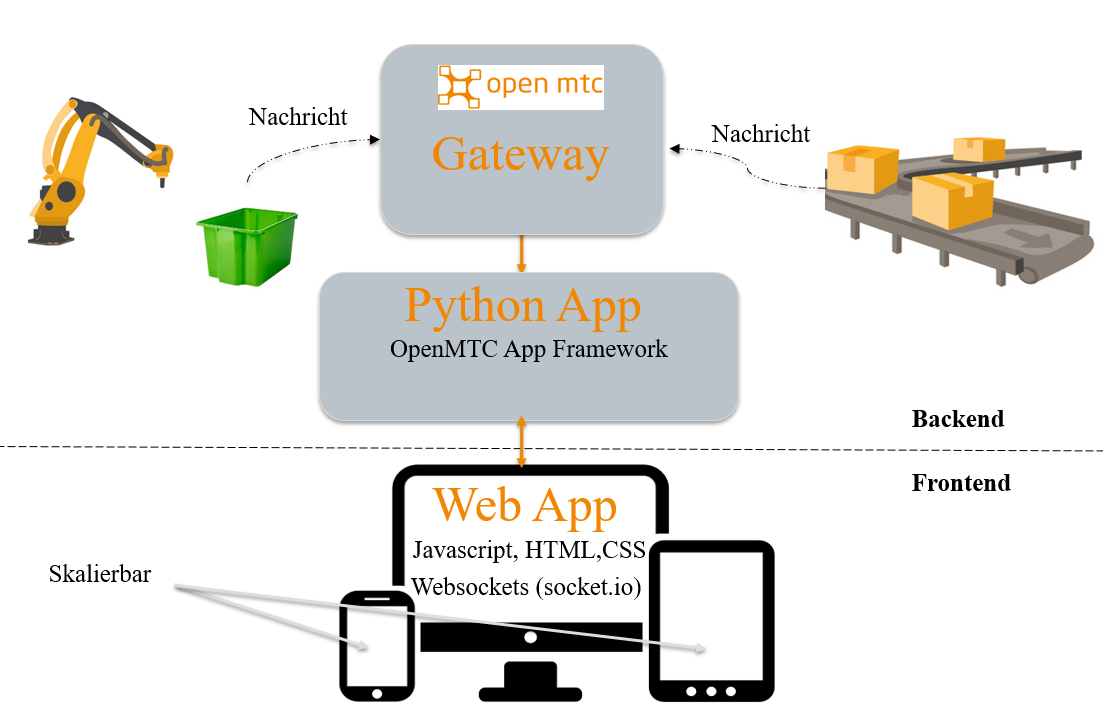
\includegraphics[width=0.9\textwidth]{concept}
\caption{Konzeption \textbf{(Bildquellen: the-mtc.org, iot.do, fotolia.com)}}
\label{concept}
\end{figure}
\subsubsection*{Frontend}
Auf Frontend Seite wird eine Webapplikation implementiert, welche die Daten in angemessener Art und Weise darstellt. Dazu müssen die schon formatierten Maschinennachrichten mittels Javascript ausgelesen und auf in den jeweiligen Bereichen dargestellt werden. Dies wird im Detail im Kapitel 'Implentierung - Frontend' erläutert. Die Webapplikation wird dabei so implementiert, dass sie skalierbar ist und somit auch auf kleineren Geräten wie Handys oder Tablets benutzt werden kann.
Damit wird, wie üblich, HTML für das Grundgerüst, Javascript für die Funktionalität und CSS zur ansprechenden Gestaltung der Website benutzt. 
\newpage
\section{Implementierung}
In diesem Kapitel wird die Implementierung des Konzeptes näher beschrieben. Dies erfolgt primär mit Ablaufdiagrammen sowie relevanten Codeauschnitten. Der Quellcode des gesamten Projektes kann auf Nachfrage bereitgestellt werden. Zu erwähnen ist, dass alle Ablaufdiagramme auf englisch sind, um eine intuitive Analogie zum Quellcode herzustellen, weil Funktionen im Quellcode größtenteils durch gleichnamige Blöcke im Diagramm dargestellt sind.
\subsection{Backend}
Um eine Testumgebung zu schaffen wurde mithilfe der auf openmtc.org verfügbaren Sensor Demo Applikationen, eine Maschinenumgebung emuliert. Es wurden die Demo Applikationen so erweitert, dass diese den Maschinennachrichten entsprechend, SID, RID, eine zufällige Nachricht und alle im Netz befindlichen Komponenten bereits in einem JSON Format an das Frontend senden. Dies geschieht außerdem von verschiedenen Containeradressen. Somit konnte insbesondere der Frontend Code auch außerhalb des Labors getestet werden. 
Innerhalb des Labors mussten dann lediglich die Adressen der Datencontainer angepasst sowie die Routinen zur Extraktion der RDF codierten Daten implementiert werden. (Dazu im Kapitel 'reale Maschinenumgebung' mehr) 
Da der Backend Code der realen Maschinenumgebung auf dem Backend Code der emulierten Umgebung aufbaut wird erst auf letzteren eingegangen. 
\newpage
\subsubsection{Emulierte Maschinenumgebung}
\subsubsection*{Erzeugung emulierter Maschinennachrichten}
Das Ablaufdiagramm zur Erzeugung der emulierten Maschinennachrichten ist in Abbildung \ref{ab1} zu erkennen. Dieses besteht aus zwei Teilen: dem Erstellen der willkürlich gewählten Maschinen und den zufälligen Nachrichten sowie der Prozessierung dieser Daten. Letzterer Punkt umfasst die Erstellung einer Containerstruktur sowie dem Senden der Daten an das Gateway. 
\begin{figure}[H]
\centering
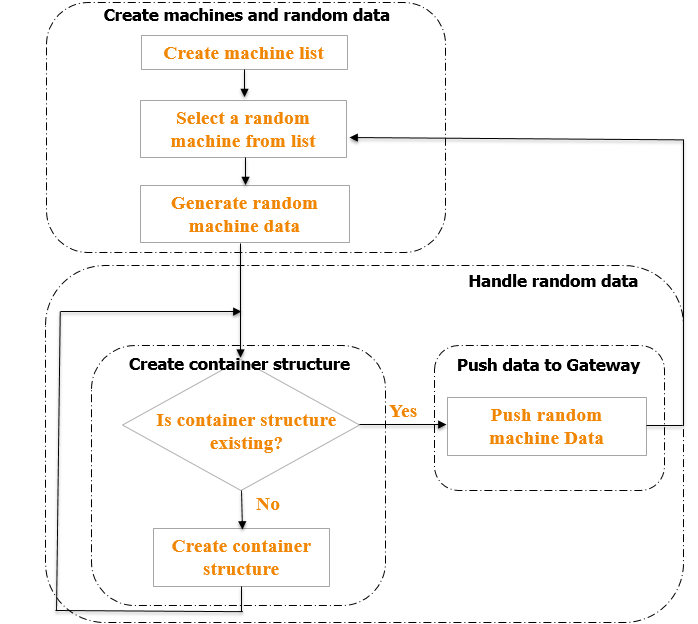
\includegraphics[width=0.7\textwidth, height= 300px]{demo}
\caption{Programmablaufplan zur Erzeugung einer emulierten Maschinenumgebung}
\label{ab1}
\end{figure}
Die Erstellung der Maschinen geschieht im Block \textbf{Create machine list}, woran sich die zufällige Auswahl eines dieser Maschinen anschließt. Darauffolgend werden die zufälligen Nachrichten in \textbf{Generate random machine data} erzeugt. Es wird zunächst überprüft, ob die Maschine bereits eine Containerstruktur für Daten dieser Maschine besitzt. Falls dies nicht der Fall ist, wird erst eine solche innerhalb des Blockes \textbf{Create container structure} erstellt um die Daten in diesen Container zu senden (Block \textbf{Push random machine data}. Dabei wird ein für die Container ein Label gewählt. Dies ist für das später behandelte Backend wichtig. Die Routine startet, dann bei der zufälligen Auswahl der nächsten Maschine (Block \textbf{Select random machine}), von neuem.
\newpage
\subsubsection*{Empfangen der emulierten Maschinennachrichten und senden an das Frontend}
Die emulierten Maschinennachrichten müssen, wie in der realen Umgebung später auch, von einem Backend empfangen und an das Frontend weitergeleitet werden. Dazu wird das Ablaufdiagramm in Abbildung \ref{ab2} betrachtet.


\begin{figure}[H]
\centering
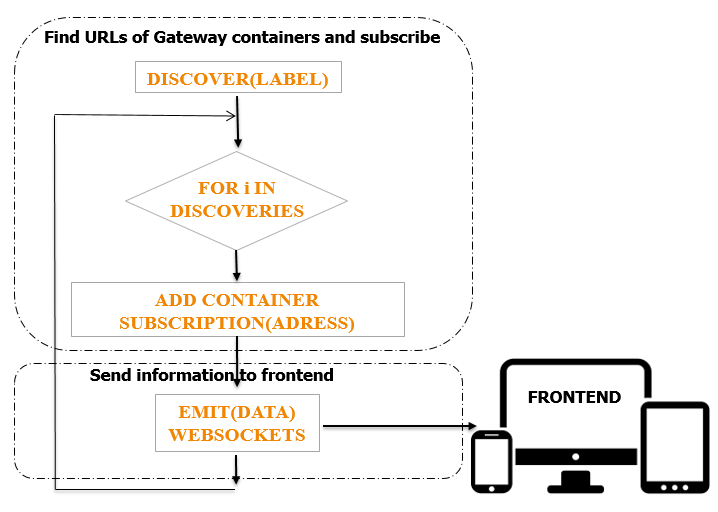
\includegraphics[width=0.9\textwidth]{backendDemo}
\caption{Programmablaufplan des Backendes zur Vermittlung der Maschinendaten an das Frontend}
\label{ab2}
\end{figure}
Zuerst werden im Block \textbf{DISCOVER(LABEL)} alle Adressen der Container mit dem angegeben Label gesucht und in einer Liste zurückgegeben. Die Label wurden dabei für alle Nachrichtencontainer innerhalb der emulierten Umgebung gleich gewählt, sodass alle erkannt werden. Anschließend wird mit einer Schleife über alle gefundenen Adressen iteriert und die $add_container_subscription()$ Funktion angewandt, womit auf jede dieser Container subskribiert wird. Innerhalb dieser Subskribierungsfunktion wird als Handler Funktion die emit() Funktion verwendet, welche die JSON Daten direkt an das Frontend sendet.
\newpage
\subsubsection{Reale Maschinenumgebung}
Der Backend Code zur Verwendung innerhalb der realen Maschinenumgebung muss in Bezug zum oben behandelten Demo Code, noch um folgende Routinen erweitert werden:
\begin{itemize}
\item Routine zur Extraktion der RDF codierten Maschinennachrichten und Aufbereitung der Nachricht im JSON Format
\item Routine zur Extraktion der RFD codierten Information über die tatsächlichen Namen der Komponenten.
\end{itemize}
\subsubsection*{Extraktion der RDF-codierten Maschinennachrichten}
Die Extraktion der Maschinennachrichten wird im folgenden Codeauschnitt implementiert.

\begin{lstlisting}[caption={Extraktion der RDF codierten Maschinennachrichten}, label=hi]
		    #create graph variable
        msg_graph = Graph()
        #append data, which is in json-ld(in a graph) to our graph
        msg_graph.parse(data=data, format='json-ld')
        
        #get adress of message
        msg_uri = msg_graph.value(predicate=RDF.type,
        object=self.ns2.Message) 
        
        # extract data from graph branches
        SID = msg_graph.value(msg_uri, self.ns2.SID)
        RID = msg_graph.value(msg_uri, self.ns2.RID)
        TRN = msg_graph.value(msg_uri, self.ns2.TRN) 
\end{lstlisting}
Dabei werden die bereits in der Theorie erläuterten Funktionen der rdf-Bibliothek benutzt. Mit $Graph()$ wird eine Graph-Variable erstellt, mit der ein Graph aufgenommen werden kann. Die Aufnahme des Graphen der Maschinendaten passiert mit der Funktion $parse$, wobei die Daten (data), analog wie bereits in der Demo Umgebung bereits erläutert, von der Subskiptionsfunktion geliefert werden und als format json-ld angegeben wird, da die Maschinendaten auch in diesem Format gesendet werden. Anschließend wird dem Graphen der Maschinendaten, die gesendete Nachricht mit $value$ entnommen. In diesem liegen wiederum die für das Frontend relevanten Information SID (Sender), RID (Empfänger) und TRN (Nachricht), welche ebenfalls mit $value$ entnommen werden.

\subsubsection*{Extraktion der tatsächlichen Komponentennamen}
Weiterhin muss für die richtigen Namen der Komponenten auf ein Manifest zurückgegriffen werden. Dieses befindet sich ebenfalls innerhalb der Containerstruktur, sodass durch die entsprechende Adresse, die richtigen Namen der Komponenten mit einen $get\_content()$ Aufruf abgerufen werden kann. Auch diese Informationen sind RDF-codiert, sodass diese, wie schon bei den Maschinennachrichten, mit den Funktionen Graph(), parse() und value(), aus dem Graphen extrahiert werden können.
\subsubsection*{Programmablaufdiagramm}
Der Teilbereich "Find URLs of Gateways and subscribe" im Ablaufdiagramm in Abbildung \ref{diare} wurde bereits für die Demo Umgebung behandelt und funktioniert analog.
Die beiden oben behandelten Zusatzroutinen können \ref{diare} im dem \textbf{ENCODE(DATA)} Block zugeordnet werden. Der Block \textbf{JSONIFY(DATA)} beinhaltet die Aufbereitung der gewonnenen Informationen in einem JSON Konstrukt. Dies wird mit Folgendem Codeauschnitt implementiert.
\begin{lstlisting}[caption={Aufbereitung der gewonnenen Informationen im JSON Format}, label=hi]
		   msg = {
            'sid': SID,
            'value': TRN,
            'rid': RID,
            'type': 'Message:',
            'devices': dev_list
        }
\end{lstlisting}
Die Liste $dev\_list$ beinhaltet alle Komponenten im Netz. An diese wird dabei immer eine Komponente mit append() angefügt, welches eine Nachricht sendet und noch nicht in der Liste vorhanden ist.

\begin{figure}[H]
\centering
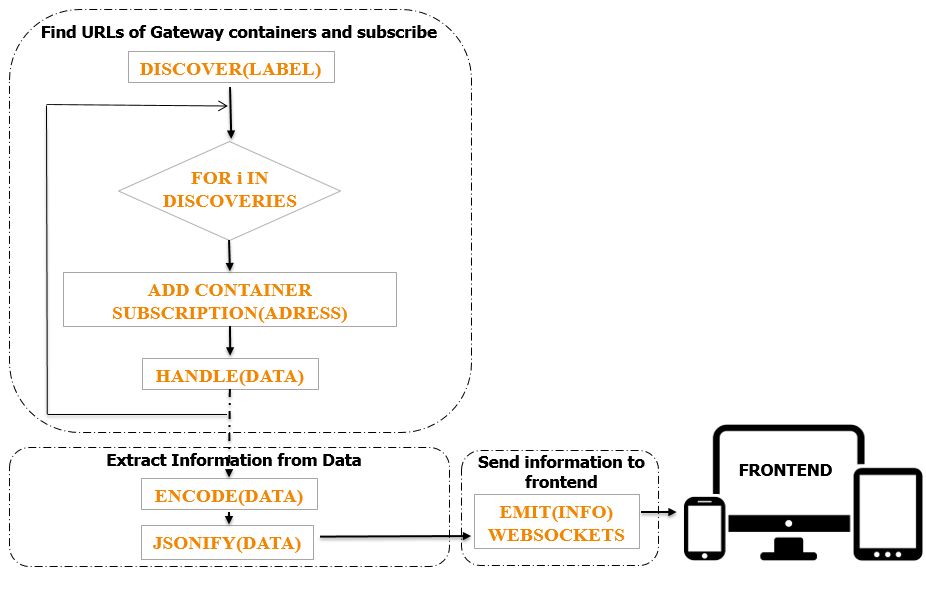
\includegraphics[width=0.9\textwidth]{backend}
\caption{Programmablaufplan des Backendes zur Vermittlung der Maschinendaten an das Frontend}
\label{diare}
\end{figure}
Der Block \textbf{EMIT(INFO)} sendet mit der emit() Funktion der socket.io Bibliothek, dann die aufbereiteten Daten an das Frontend. 
\newpage

\subsection{Frontend}

\section{Zusammenfassung}
Insgesamt wurde die Konzepte der Theorie verstanden und im Projekt erfolgreich angewandt.
Damit konnten die anfangs definierten Ziele für das Projekt erreicht. Es konnte eine Web basierte Applikation zur Visualisierung der Kommunikation des betrachteten Prozesses implementiert werden, welche auch die Möglichkeit bietet, alle Netzwerkkomponenten zu sehen. Zusätzlich dazu wurde eine Filter Funktion implementiert um die Kommunikation aus Sicht einer Komponente anzuzeigen. Entsprechend wurde für diesen Fall auch das Design des Chat Raums angepasst. Die Funktionalität der Applikation konnte im Labor erfolgreich getestet werden. Weiterhin wurde für Testzwecke eine emulierte Maschinenumgebung mithilfe der verfügbaren Demo Applikationen geschaffen, welche es erlaubt auch außerhalb des Labors, die Funktionalität zu überprüfen sowie neue Ansätze auszutesten. Somit wurde eine Grundlage für weitere Projekte und Implementierungen geschaffen. 
\section{Ausblick}
\section{Anhang}



%--------------------------------------------------------------------
%%%%%%%%%%%%%%%%%%%%%%%%%%%%%%%%%%%%%%%%%%%%%%%%%%%%%%%%%%%%%%%%%%%%%%%%%%%%%%%%%%%%%%%%%%%%%%%%%%%literatur
% Abschließend sind die Quellen von Bildern und Zitaten nicht zu vergessen.
\newpage

\bibliographystyle{plain}
% argument is your BibTeX string definitions and bibliography database(s)
\bibliography{references}

%\begin{thebibliography}{}   
%\bibitem{en_ue5}          % Hier beginnt das Literaturverzeichnis
%Abbildung 1: Kai Strunz, Felix Klein und Peter Teske,                            % Autoren
%\newblock {\textit{Übung 5 - Quellen und Lasten, Elektrische Netzwerke,}}
%\newblock TU Berlin, 2014.

%\bibitem{DIN1338}
%Normenausschuss Technische Grundlagen (NATG) im DIN,                         % Autoren
%\newblock {\textit{DIN 1338:2011-03, Formelschreibweise und Formelsatz, }}
%\newblock DIN Deutsches Institut für Normung e. V., Berlin, 2011-03.

%\bibitem{Abbildung_2}
%Abbildung 2:	Erika Musterfrau, Dörte Shakira Wagner,
%\newblock {\it  Anzugsmomente von Kolbenrückholfedervorspannungsschrauben,}
%\newblock TU Berlin, 2014.

%\bibitem{Informationen}
%Claire Grube, Rainer Wahnsinn und Kurt Zschluß 
%\newblock {\it Praktikumsbeschreibung Kurbelwelleninnenrandbeleuchtung,}
%\newblock TU Berlin, 2014.
%\end{thebibliography}
%%%%%%%%%%%%%%%%%%%%%%%%%%%%%%%%%%%%%%%%%%%%%%%%%%%%%%%%%%%%%%%%%%%%%%%%%%%%%%%%%%%%%%%%%%%%%%%%%%%%%
%--------------------------------------------------------------------

\end{document}